\documentclass[12pt]{report}
\usepackage{amsmath}
\usepackage{graphicx}
\usepackage[colorlinks=true, linkcolor=black, citecolor=black, filecolor=black, urlcolor=black]{hyperref}
\usepackage{lipsum}
\usepackage{pdfpages}
\usepackage{titlesec}
\usepackage[utf8]{inputenc}
\title{Heat Production Management Project for Semester Project 2}
\author{Kacper Grzyb \and Sebestyen Deak \and Ignad Bozhinov \and Leonardo Gianola \and Levente Sohar}
\date{03-06-2024}

% Define a command to convert number section counting to alphabetical section counting
\makeatletter
\newcommand{\alphsection}{\@alph\c@section}
\makeatother

% Redefine the sectioning commands
\renewcommand{\thesection}{\thechapter\alphsection}
\titleformat{\section}
  {\normalfont\Large\bfseries}{\thesection}{1em}{}


\begin{document}
\maketitle

\tableofcontents

% Chapter 1
\chapter{Introduction}
Introduction chapter goes here

% Chapter 2
\chapter{Release Planning}
Release Planning chapter goes here

% Chapter 3
\chapter{Sprint Materials}
Sprint Planning Chapter goes here

% Chapter 4
\chapter{Technical Details}
Technical Details Chapter goes here

% Chapter 4a
\section{Software Architecture and Design}

\subsection*{Tools}
The team decided to use the ASP.NET Core framework's Razor Pages for building the project for reasons such as:
\begin{itemize}
  \item The most important argument for using ASP.NET Core is it's cross-platform functionality. The developers in the team use 
  both Macintosh and Windows based systems, therefore a framework that could switch seamlessly between them was crucial.
  \item As the name suggests, the framework runs in the .NET ecosystem, which is what the team has been taught in the course so far
  therefore it is what the team is most experienced and most comfortable working in.
  \item With Razor Pages being a web-page based solution, the UI is mostly composed of HTML and CSS, which some team members already
  had experience in and the rest was eager to learn. A light-weight, web-based solution allowed the team to be more flexible,
  and develop the app at a more rapid pace compared to if the team chose a Model-View-Controler (or a Model-View-ViewModel) solution.
  This freedom allowed for more features and better adjustment to changing the project requirements.
\end{itemize}
As for other tools, the team used:
\begin{itemize}
  \item Github: Source and Version Control, Collaborative Development of the App
  \item Jira: Task Management and Planning as well as adhearing to Agile which was one of the requirements for the project
  \item Discord: Communication and Resource Sharing
  \item diagrams.net: Creating UML Diagrams for this chapter
  \item Figma: Prototyping and General UI Design
  \item Visual Studio and Visual Studio Code: Code Editors
\end{itemize}

\subsection*{Database Architecture}
Before diving into the program architecture the in-memory database solution offered by Razor Pages must first be mentioned.
In order to achieve data persistance while switching in between pages in a Razor Pages project, a database must be used. 
Since we did not want to go too far out of the scope of the project, we decided not to use a dedicated database solution
like a MySQL or MSSQL Server for this project, expecially because the team has not had any database modeling courses
yet. Instead we chose a middle-ground, which is the before mentioned in-memory database. This soultion offers similar functionality
to a real database, with the comfort of running in the program's memory, which eliminates potential connection, authentication
privilege and/or security risks and issues connected with using databases.
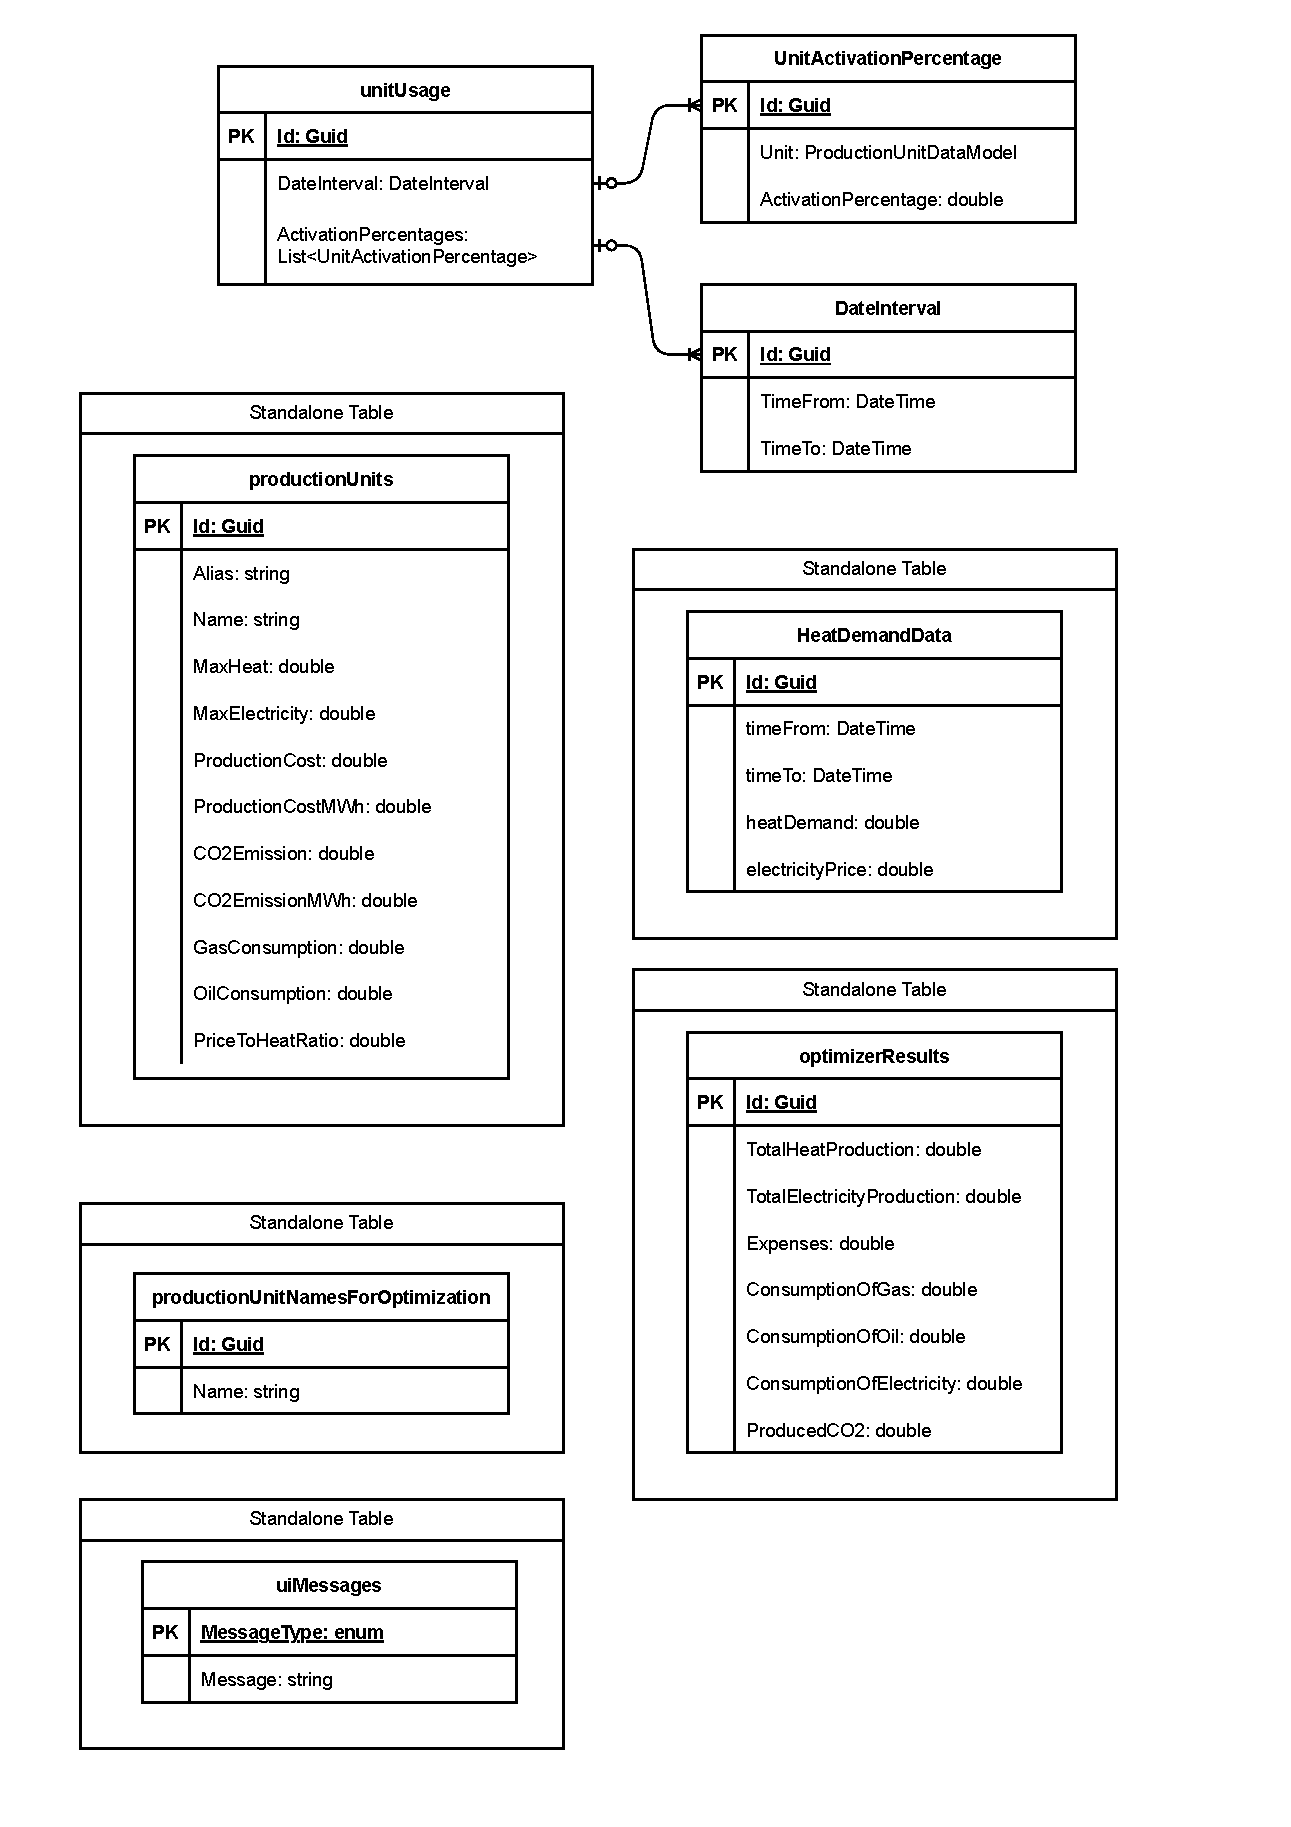
\includepdf[pages=-]{Resources/SP2-database-diagram.pdf}
The database does not fully comply to standard database structures one could see when dealing with real database systems. 
We do see the limitations of this design and the flaws inside of it, such as the lack of connections between tables and the 
lack of foreign keys inside of each table. Instead some fields in the tables use custom class data types for ease of use. Despite the flaws
of using DbSets, we found that their functionality was sufficient for the scope of the project. It is also worth to mention, that due
to our lack of experience with Razor Pages, we were unsure of how DbSets and in-memory data structures function. Because of that in the
middle of development the database had to be refactored from a more json-like data storage structure to one that complies
with standards enforced by DbSets, such as using Primary Keys. It is because of this process that we ended up having a mixture of both structures.

\subsection*{Applicaion Flow}
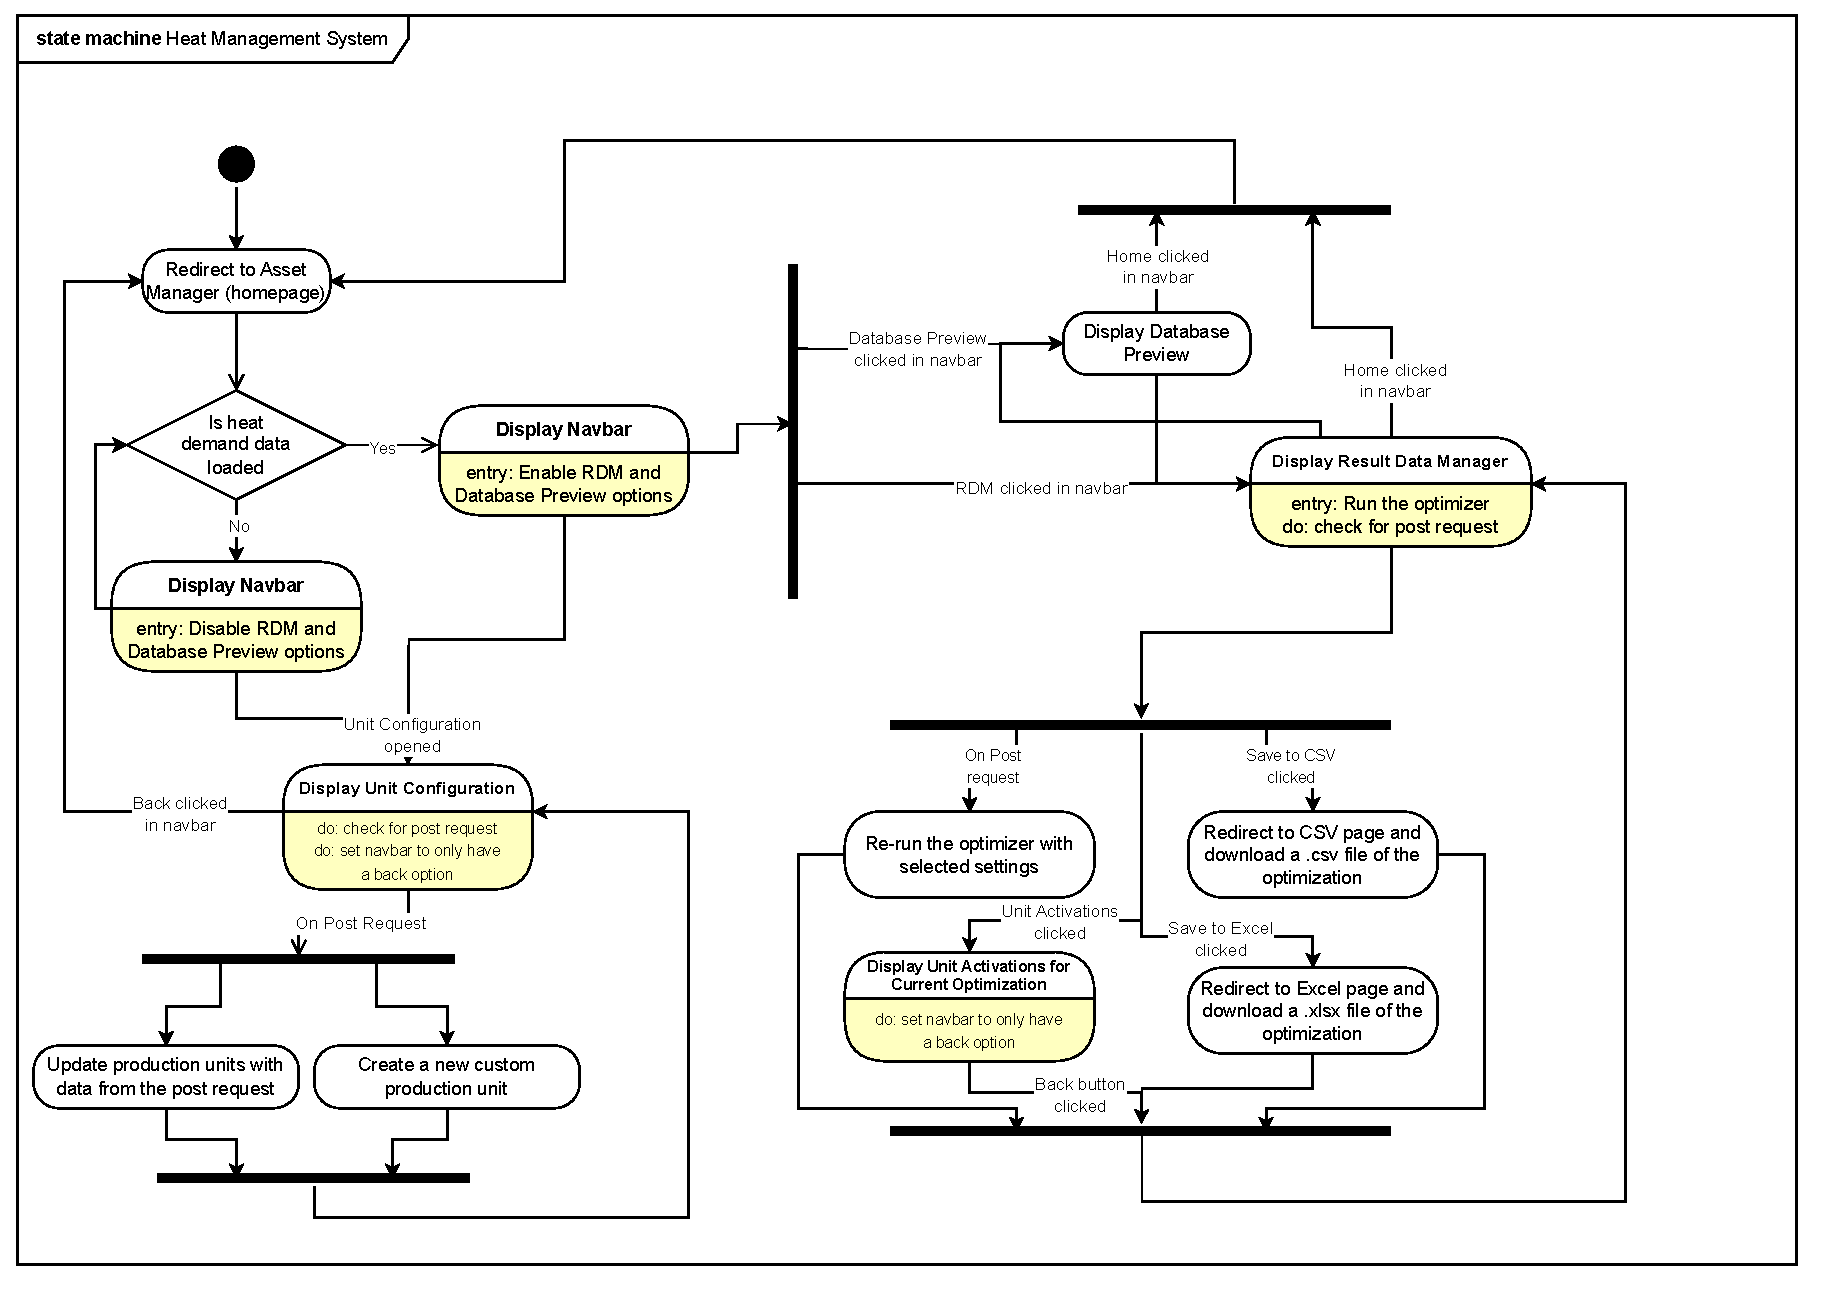
\includepdf[pages=-]{Resources/SP2-state-machine.pdf}

% Chapter 4b
\section{Simple Design}
Simple design yapping goes here

% Chapter 4c
\section{Incremental Design}
Incremental Design yapping goes here

% Chapter 4d
\section{Refactoring}
Refactoring yapping goes here

% Chapter 4e
\section{Test-Driven Development}
Test-Driven Development yapping goes here

% Chapter 4f
\section{Unit Testing}
Unit Testing yapping goes here

% Chapter 4g
\section{Pair Programming}
Pair Programming yapping goes here

% Chapter 4h
\section{Code Review}
Code Review yapping goes here

% Chapter 5
\chapter{Conclusion and Group's Reflections}
Conclusion chapter goes here

% Chapter 5a
\section{Working on a common project with other groups}
5a yapping goes here

% Chapter 5b
\section{What went well and not so well with the group's specific set of tasks}
5b yapping goes here

% Chapter 5c
\section{Specific contributions of each team member}
5c yapping goes here

\section{Future actions to prevent problems and difficulties faced during the project}
5d yapping goes here


\end{document}